% --------------------------------------------------------------------------------
\newpage
\section{Pitch Completion Module}
% --------------------------------------------------------------------------------

% Make general target
\hypertarget{Concepts:PitchCompletionModule}{}

% Make target for following functions:
\hypertarget{Concepts:IPEMPeriodicityPitch}{}

\subsection{Introductory description}
% --------------------------------------------------------------------------------

The Pitch Completion Module (PCM) calculates the periodicity pitch
image of a signal. Strictly speaking, the neural rate code of the
auditory nerve images is taken as input and a periodicity analysis
is the output. Otherwise stated, the inputs are primary images and
the outputs are pitch images. In our global chart of image
transformation modules PCM is localized in the section on
perception (fig. \ref{Fig:ModulesPCM}).
\begin{figure}[h]
    \centering
    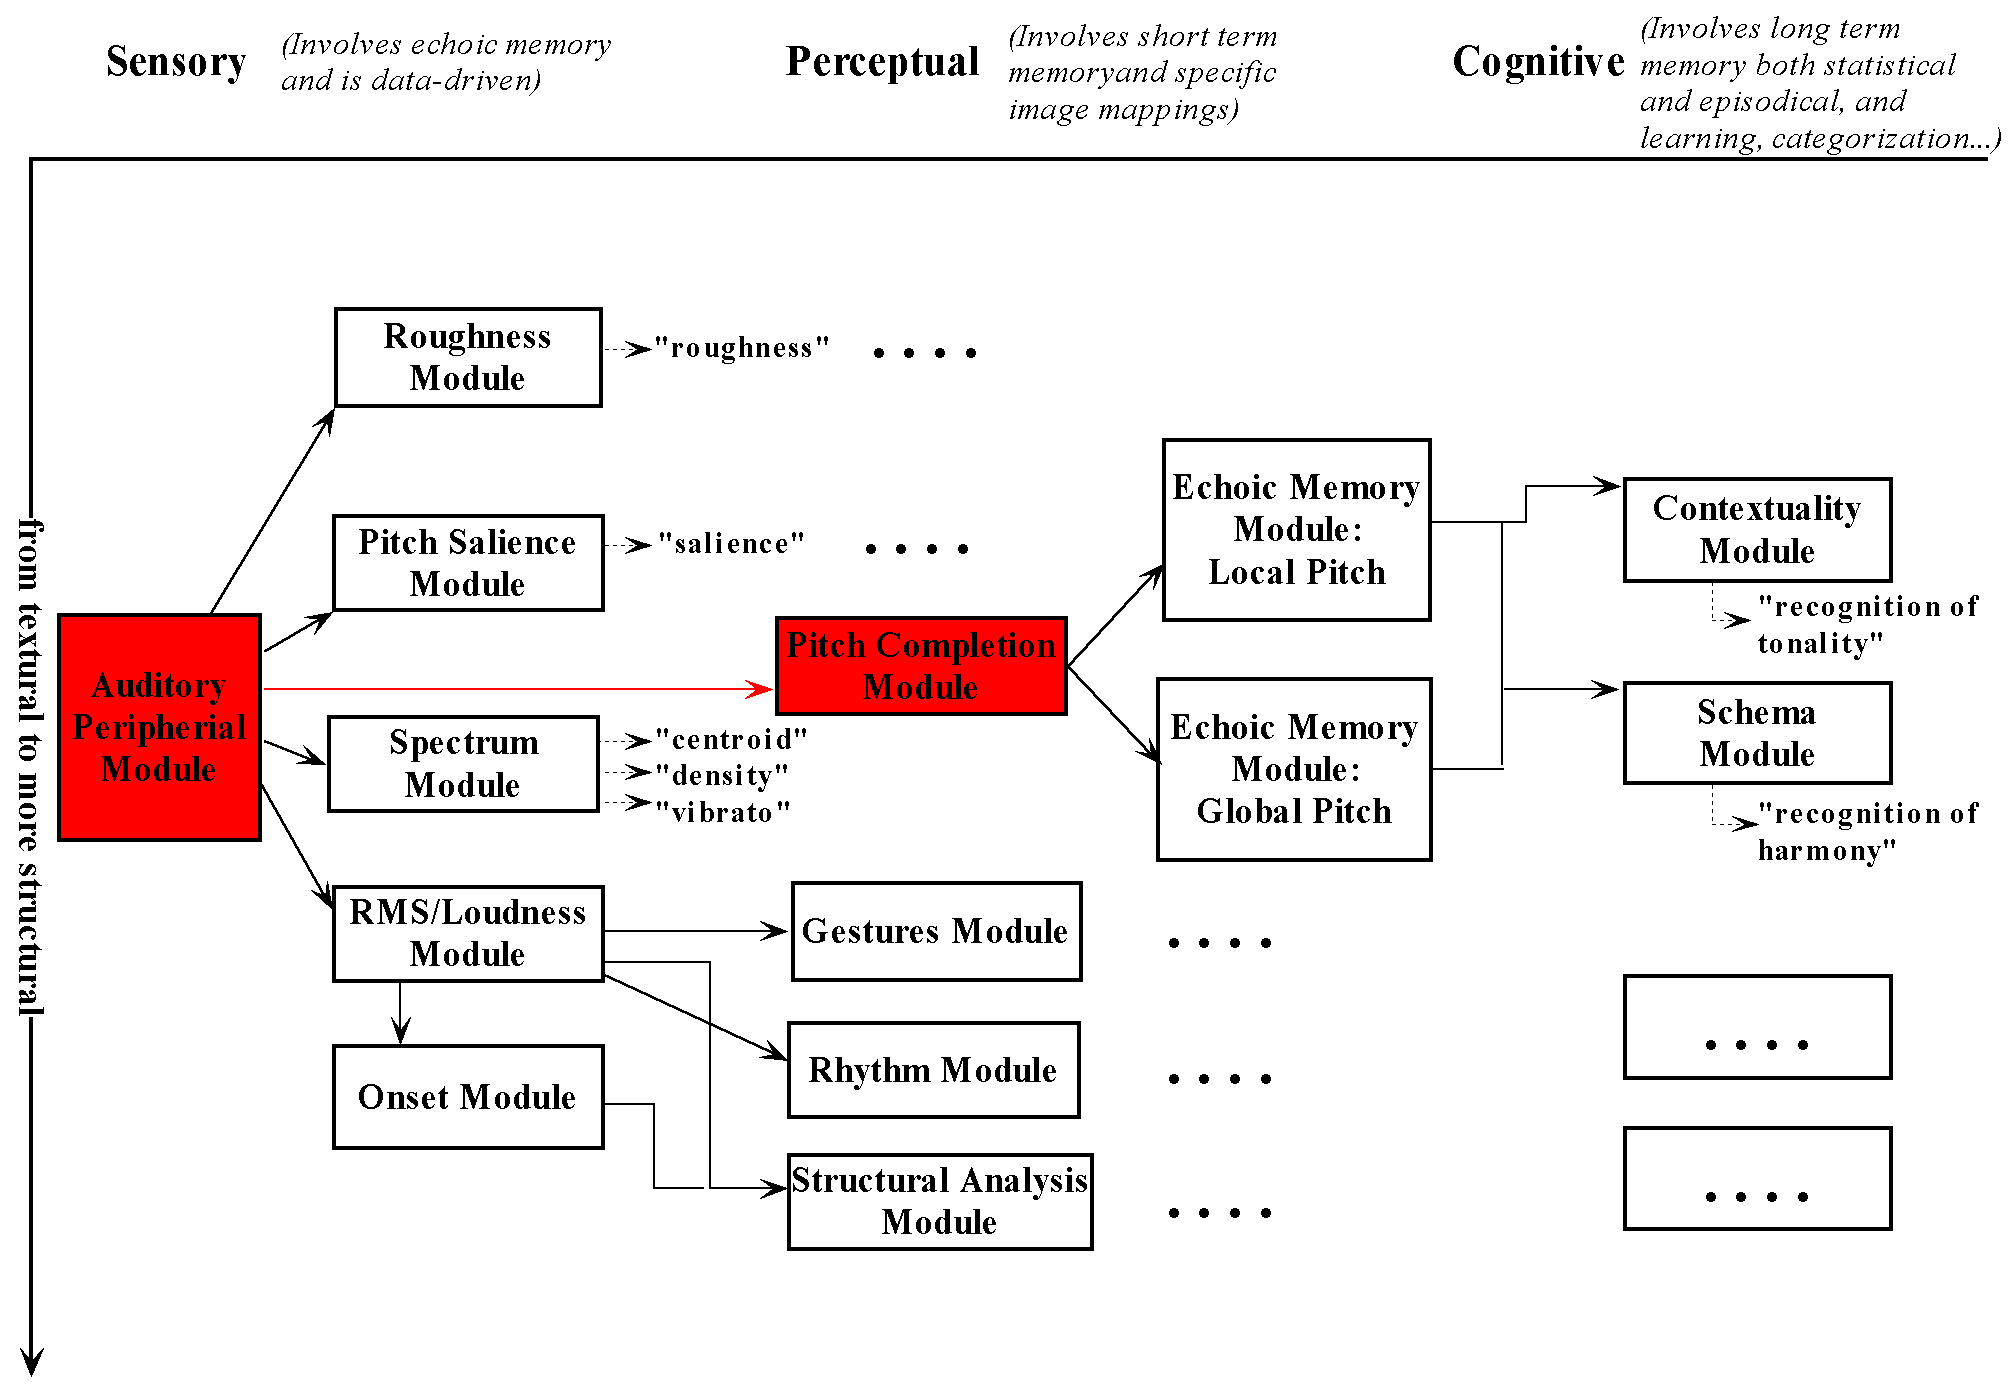
\includegraphics[width=\textwidth]{Graphics/ModulesPCM}
    \caption{Chart of image transformation modules, with PCM highlighted}
    \label{Fig:ModulesPCM}
\end{figure}

A periodicity analysis of primary images is dealt with at
different occasions, such as in
\hyperlink{Concepts:RhythmModule}{rhythm}. The main difference is
the focus of attention. In rhythm periodicity we look at larger
periodicities than in pitch where the focus of our attention is
between 80 and 1250 Hz.
\begin{itemize}
\item
    The lower limit of 80 Hz accounts for the fact that for smaller frequencies,
    the sensation of pitch becomes more a sensation of textural properties.
    This is a shift of perceptual categorization which is taken into account
    in our modeling. Indeed, our model of \hyperlink{Concepts:RoughnessModule}{roughness}
    took into account a range of frequencies between 5 and 300 Hz but
    the focus was on frequencies between 50 and 70 Hz (see the filter characteristics
    in figure \ref{Fig:Filters}).
\item
    The higher limit of 1250 Hz is related to the limits of neural synchronization.
    Beyond about 1250 Hz, the neurons are no longer able to follow the exact
    period of the signal very accurately, and periodicity pitch becomes unreliable.
\end{itemize}
Pitch estimations at higher frequencies could rely on spectral
information contained in $e(t,c)$. Such spectral images could be
obtained by taking the RMS-values in each channel over short time
periods using \hyperlink{FuncRef:IPEMCalcRMS}{IPEMCalcRMS}.
However, the pitch information necessary to deal with harmonic
relationships, is here assumed to be contained in the time-code of
the auditory nerve images, and this within a frequency band of 80
to 1250 Hz.

From a conceptual point of view the Pitch Completion Module
performs a transformation from time-code to place-code, i.e. from
patterns whose frequency is contained within the temporal
characteristics of the pattern to patterns whose frequency is
encoded along a spatial array. Physiological evidence for
periodicity pitch perception has been gathered by
\citeA{Langner:92,Langner:97}. Figure \ref{Fig:PCMModule} shows the
modules involved in the image transformation process.
\begin{figure}[h]
    \centering
    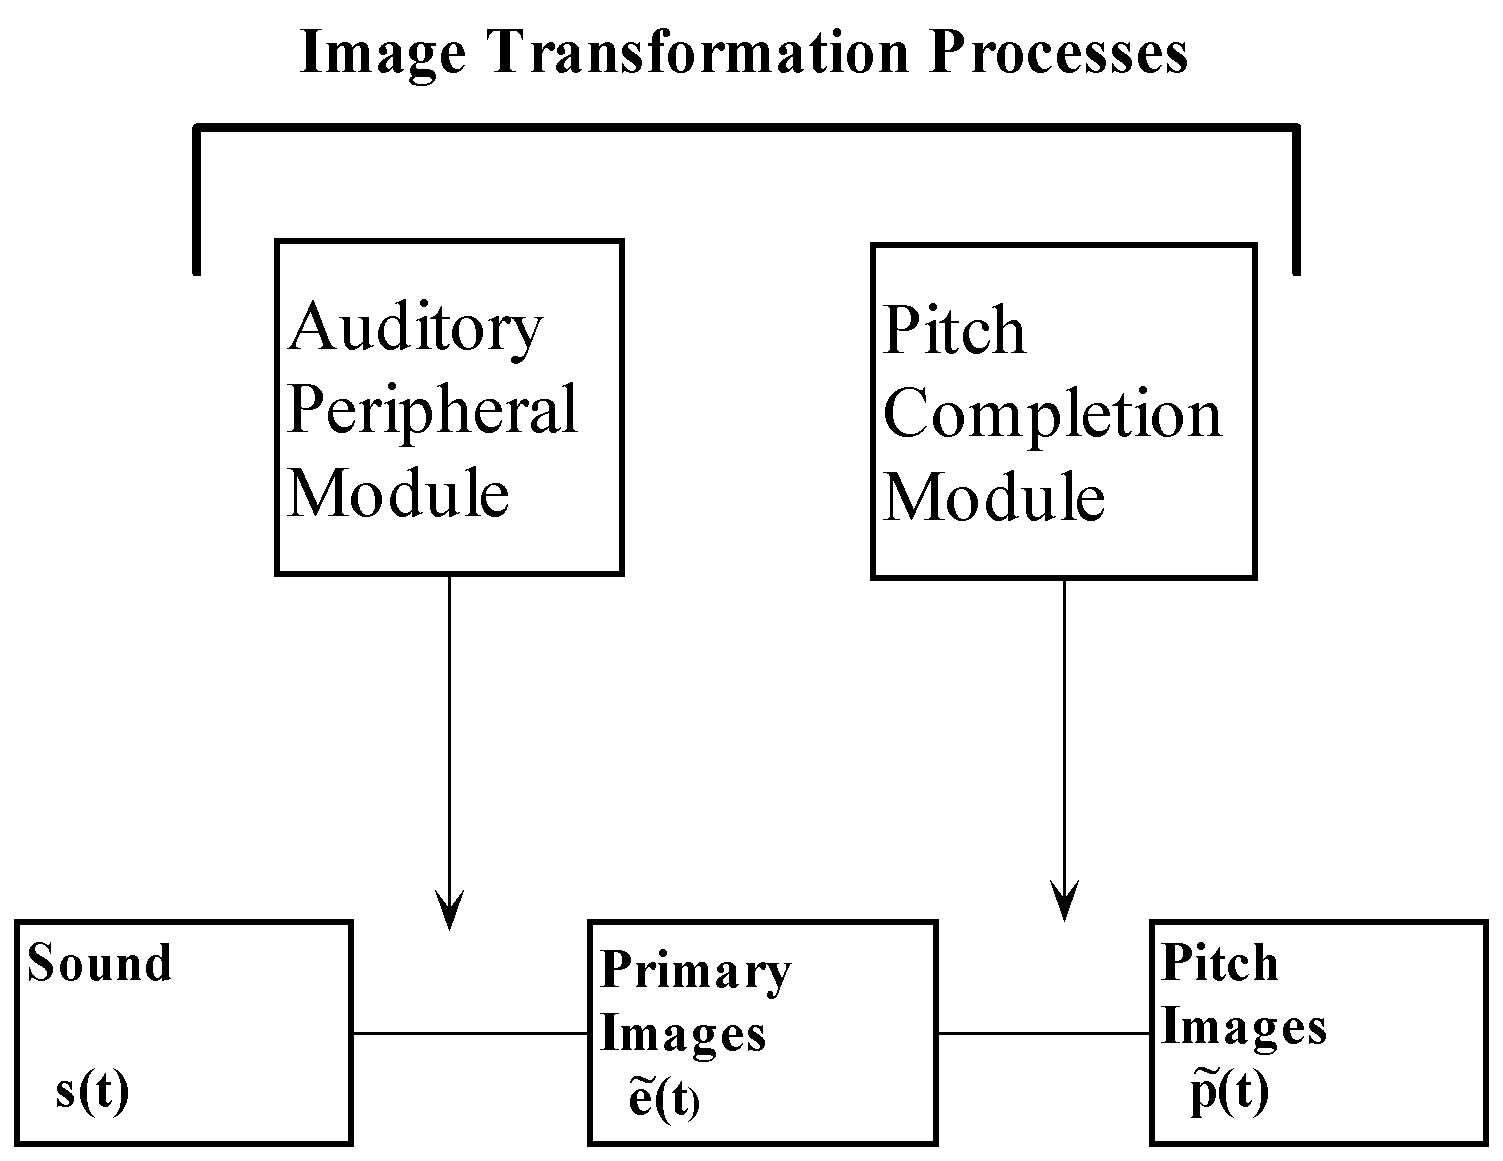
\includegraphics[width=\IPEMDefaultFigureWidth]{Graphics/PCMModule}
    \caption{Image Transformation Process: Pitch Completion Module}
    \label{Fig:PCMModule}
\end{figure}

\subsection{Functional-logical description}
% --------------------------------------------------------------------------------

First the auditory nerve images are calculated using the
\hyperlink{Concepts:AuditoryPeripheralModule}{Auditory Peripheral
Module}. The Pitch Completion Module then transforms these images
into pitch images.
\[APM:~ s(t) \rightarrow e(t,c)\]
\[PCM:~ e(t,c) \rightarrow p(t,\tau)~(=~\tilde{p}(t))\]

The Pitch Completion Module has two stages. First a periodicity
analysis of each $e(t,c)$ pattern, band-pass filtered for 80-1250
Hz, is made, where $f[e(t,c)]$ is the band-pass filtered auditory
nerve pattern for channel $c$, and $p(t,c,\tau)$ or
$\tilde{p}(t,c)$ the periodicity analysis of that pattern, with
$\tau$ denoting the period. The detected periods are registered
along a spatial array of periods. We thus have:
\begin{displaymath}
PCM1:~ \left[
\begin{array}{l}
f[e(t,1)] \\ f[e(t,2)] \\ \cdots \\ f[e(t,C)]
\end{array}
\right] \rightarrow \left[
\begin{array}{l}
\tilde{p}(t,1) \\ \tilde{p}(t,2) \\ \cdots \\ \tilde{p}(t,C)
\end{array}
\right]
\end{displaymath}

Secondly, a {\sl coincidence mechanism} sums up the
$\tilde{p}(t,c)$ over all channels patterns and stores the result
in a summary auto-correlation pattern called $\tilde{p}(t)$:
\begin{displaymath}
PCM2:~ \left[
\begin{array}{l}
\tilde{p}(t,1) \\ \tilde{p}(t,2) \\ \cdots \\ \tilde{p}(t,C)
\end{array}
\right] \rightarrow \tilde{p}(t)
\end{displaymath}

The resulting pattern $\tilde{p}$ (in alternative notation
$p(\tau)$) at time $t$ is called the pitch image or {\sl
completion image} at time $t$. The pitch is represented along the
$\tau$ axis. The completion image is related to the notion of
virtual pitch pattern. It gives an account of the common
periodicity along the auditory neurons in the frequency region of
80 Hz to 1250 Hz. Notice than the procedure outlined for PCM is
very similar to the procedure used for the detection of
periodicity in rhythm patterns, as described in the Example
section of the \hyperlink{Concepts:RhythmModule}{Rhythm Module}.

\subsection{Signal processing description}
% --------------------------------------------------------------------------------

These are the steps of the periodicity pitch calculation:

\begin{itemize}
\item Filtering\\
    The channels of the ANI are filtered between 80 and 1250 Hz. Due
    to the fact that the output of the auditory model gives the
    envelopes of the neural firing probabilities ($<$ 1250 Hz), it
    suffices to first apply a low-pass filter and then subtract that
    from the original signal in order to obtain the pitch. The
    low-pass filter is a second order Butterworth filter with a
    cutoff frequency of 80 Hz.
    \[ \tilde{e}_{filt}(t) = f[\tilde{e}(t)] \]
\item Auto-correlation\\
    A frame-based auto-correlation analysis is performed on the
    filtered channels. A frame width $FW$ and step size $FS$ are
    chosen and then for each frame and each channel $c$, we perform
    an auto-correlation for each time-lag $\delta$:
    \[
        p(t,c,\delta) = \int_{t}^{t+FW}{e_{filt,c}(\tau).e_{filt,c}(\tau+\delta).d\tau}
        \qquad \textrm{where $\delta \in [0,FW]$}
    \]
    and, by combining the results for all time lags $\delta$ in one
    vector, this gives us $\tilde{p}(t,c)$
\item Coincidence mechanism\\
    Summation of the auto-correlation results over all channels:
    \[ \tilde{p}(t) = \sum_{n=1}^{C}\tilde{p}(t,c) \]
\end{itemize}


\subsection{Implementation}
% --------------------------------------------------------------------------------

\begin{tabularx}{\linewidth}{llX}
\hyperlink{FuncRef:IPEMPeriodicityPitch}{IPEMPeriodicityPitch} & - & Calculates periodicity pitch from nerve image\\
\end{tabularx}


\subsection{Examples}
% --------------------------------------------------------------------------------

Figure \ref{Fig:SchumannPeriodicityPitch} shows the results of
first processing our familiar
\IPEMSound{Sounds/SchumannKurioseGeschichte.wav}{excerpt of
Schumann's Kuriose Geschichte} with the APM and then processing
the primary image with the Pitch Completion Module. The MATLAB
code is:\\

\begin{IPEMCodeEnvironment}
[ANI,ANIFreq,ANIFilterFreqs] = ...
\newline IPEMCalcANIFromFile('SchumannKurioseGeschichte.wav',[],[],1);
\newline [PP,PPFreq,PPPeriods,PPFANI] = IPEMPeriodicityPitch(ANI,ANIFreq,[],[],[],1);
\end{IPEMCodeEnvironment}\\

where \IPEMCodeExtract{PPFANI} are the filtered (between 80-1250
Hz) auditory nerve images.\\

Figure \ref{Fig:ShepardCChordPeriodicityPitch} shows the results
of first processing the \IPEMSound{Sounds/ShepardCChord.wav}{C
major chord using Shepard tones} with the APM and then processing
the primary image with the Pitch Completion Module.

\begin{figure}[h]
    \centering
    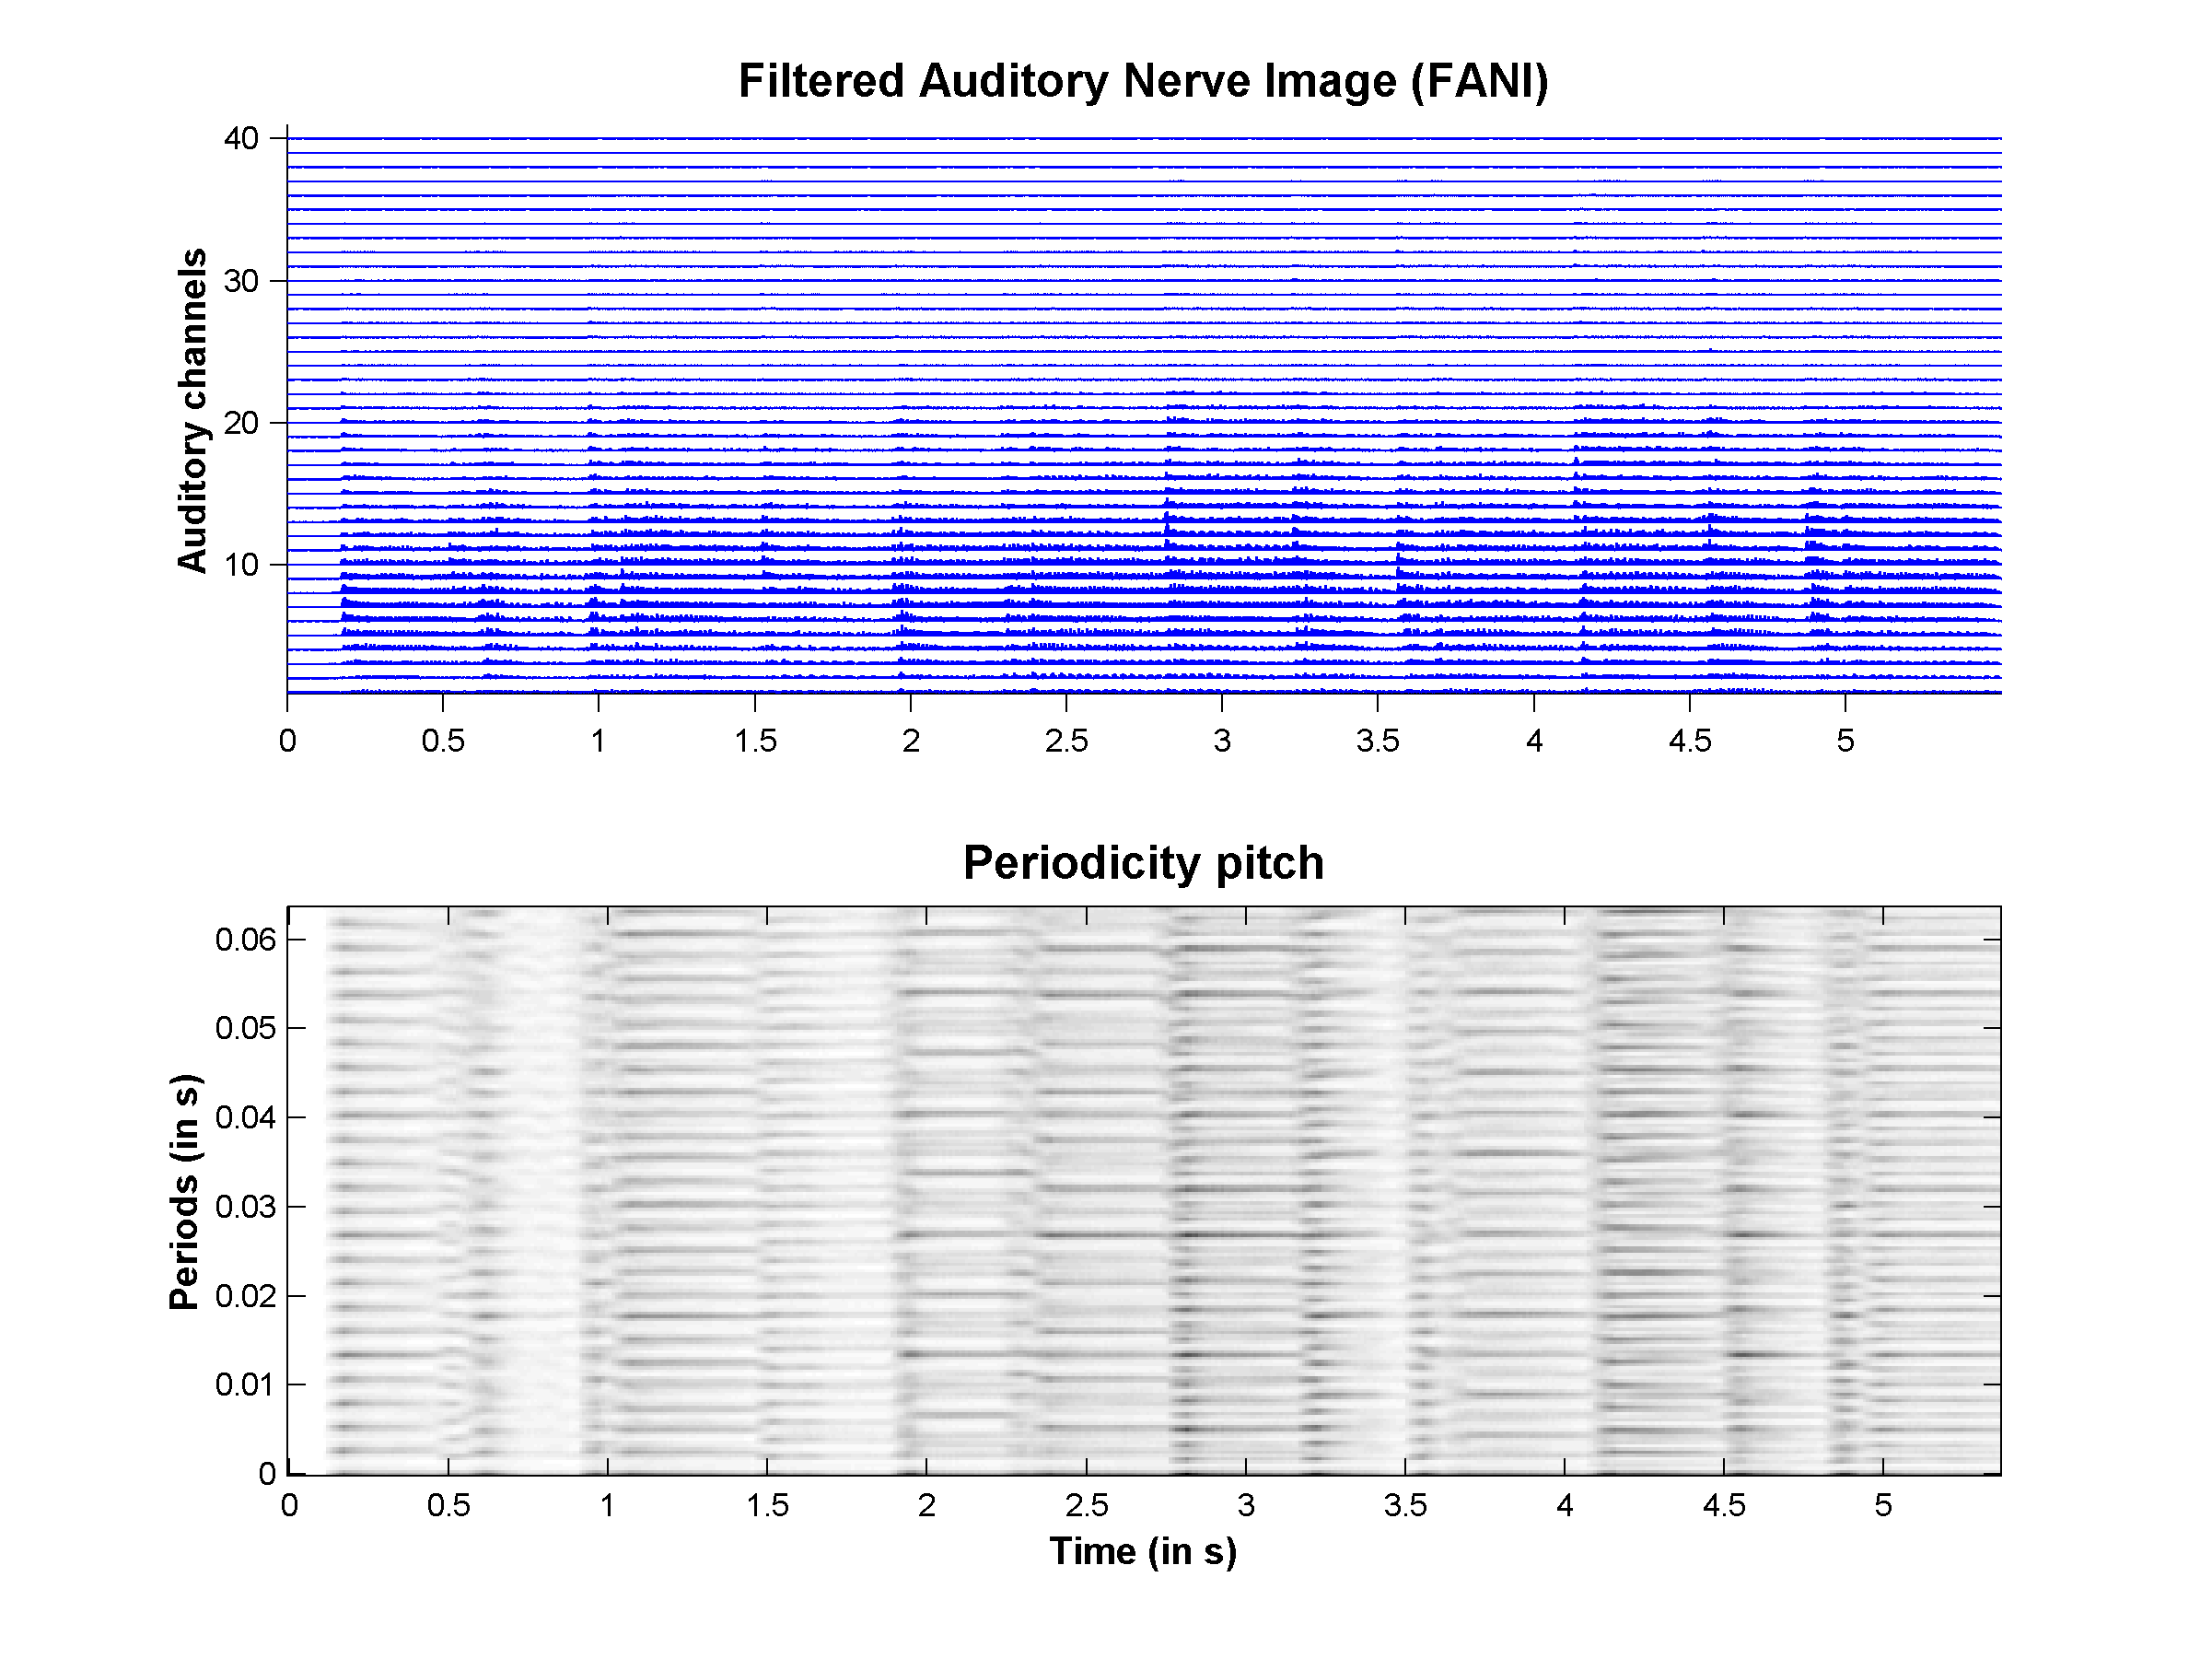
\includegraphics[width=\IPEMDefaultFigureWidth]{Graphics/SchumannPeriodicityPitch}
    \caption{Periodicity Pitch for the excerpt of Schumann's Kuriose Geschichte}
    \label{Fig:SchumannPeriodicityPitch}
\end{figure}

\begin{figure}[h]
    \centering
    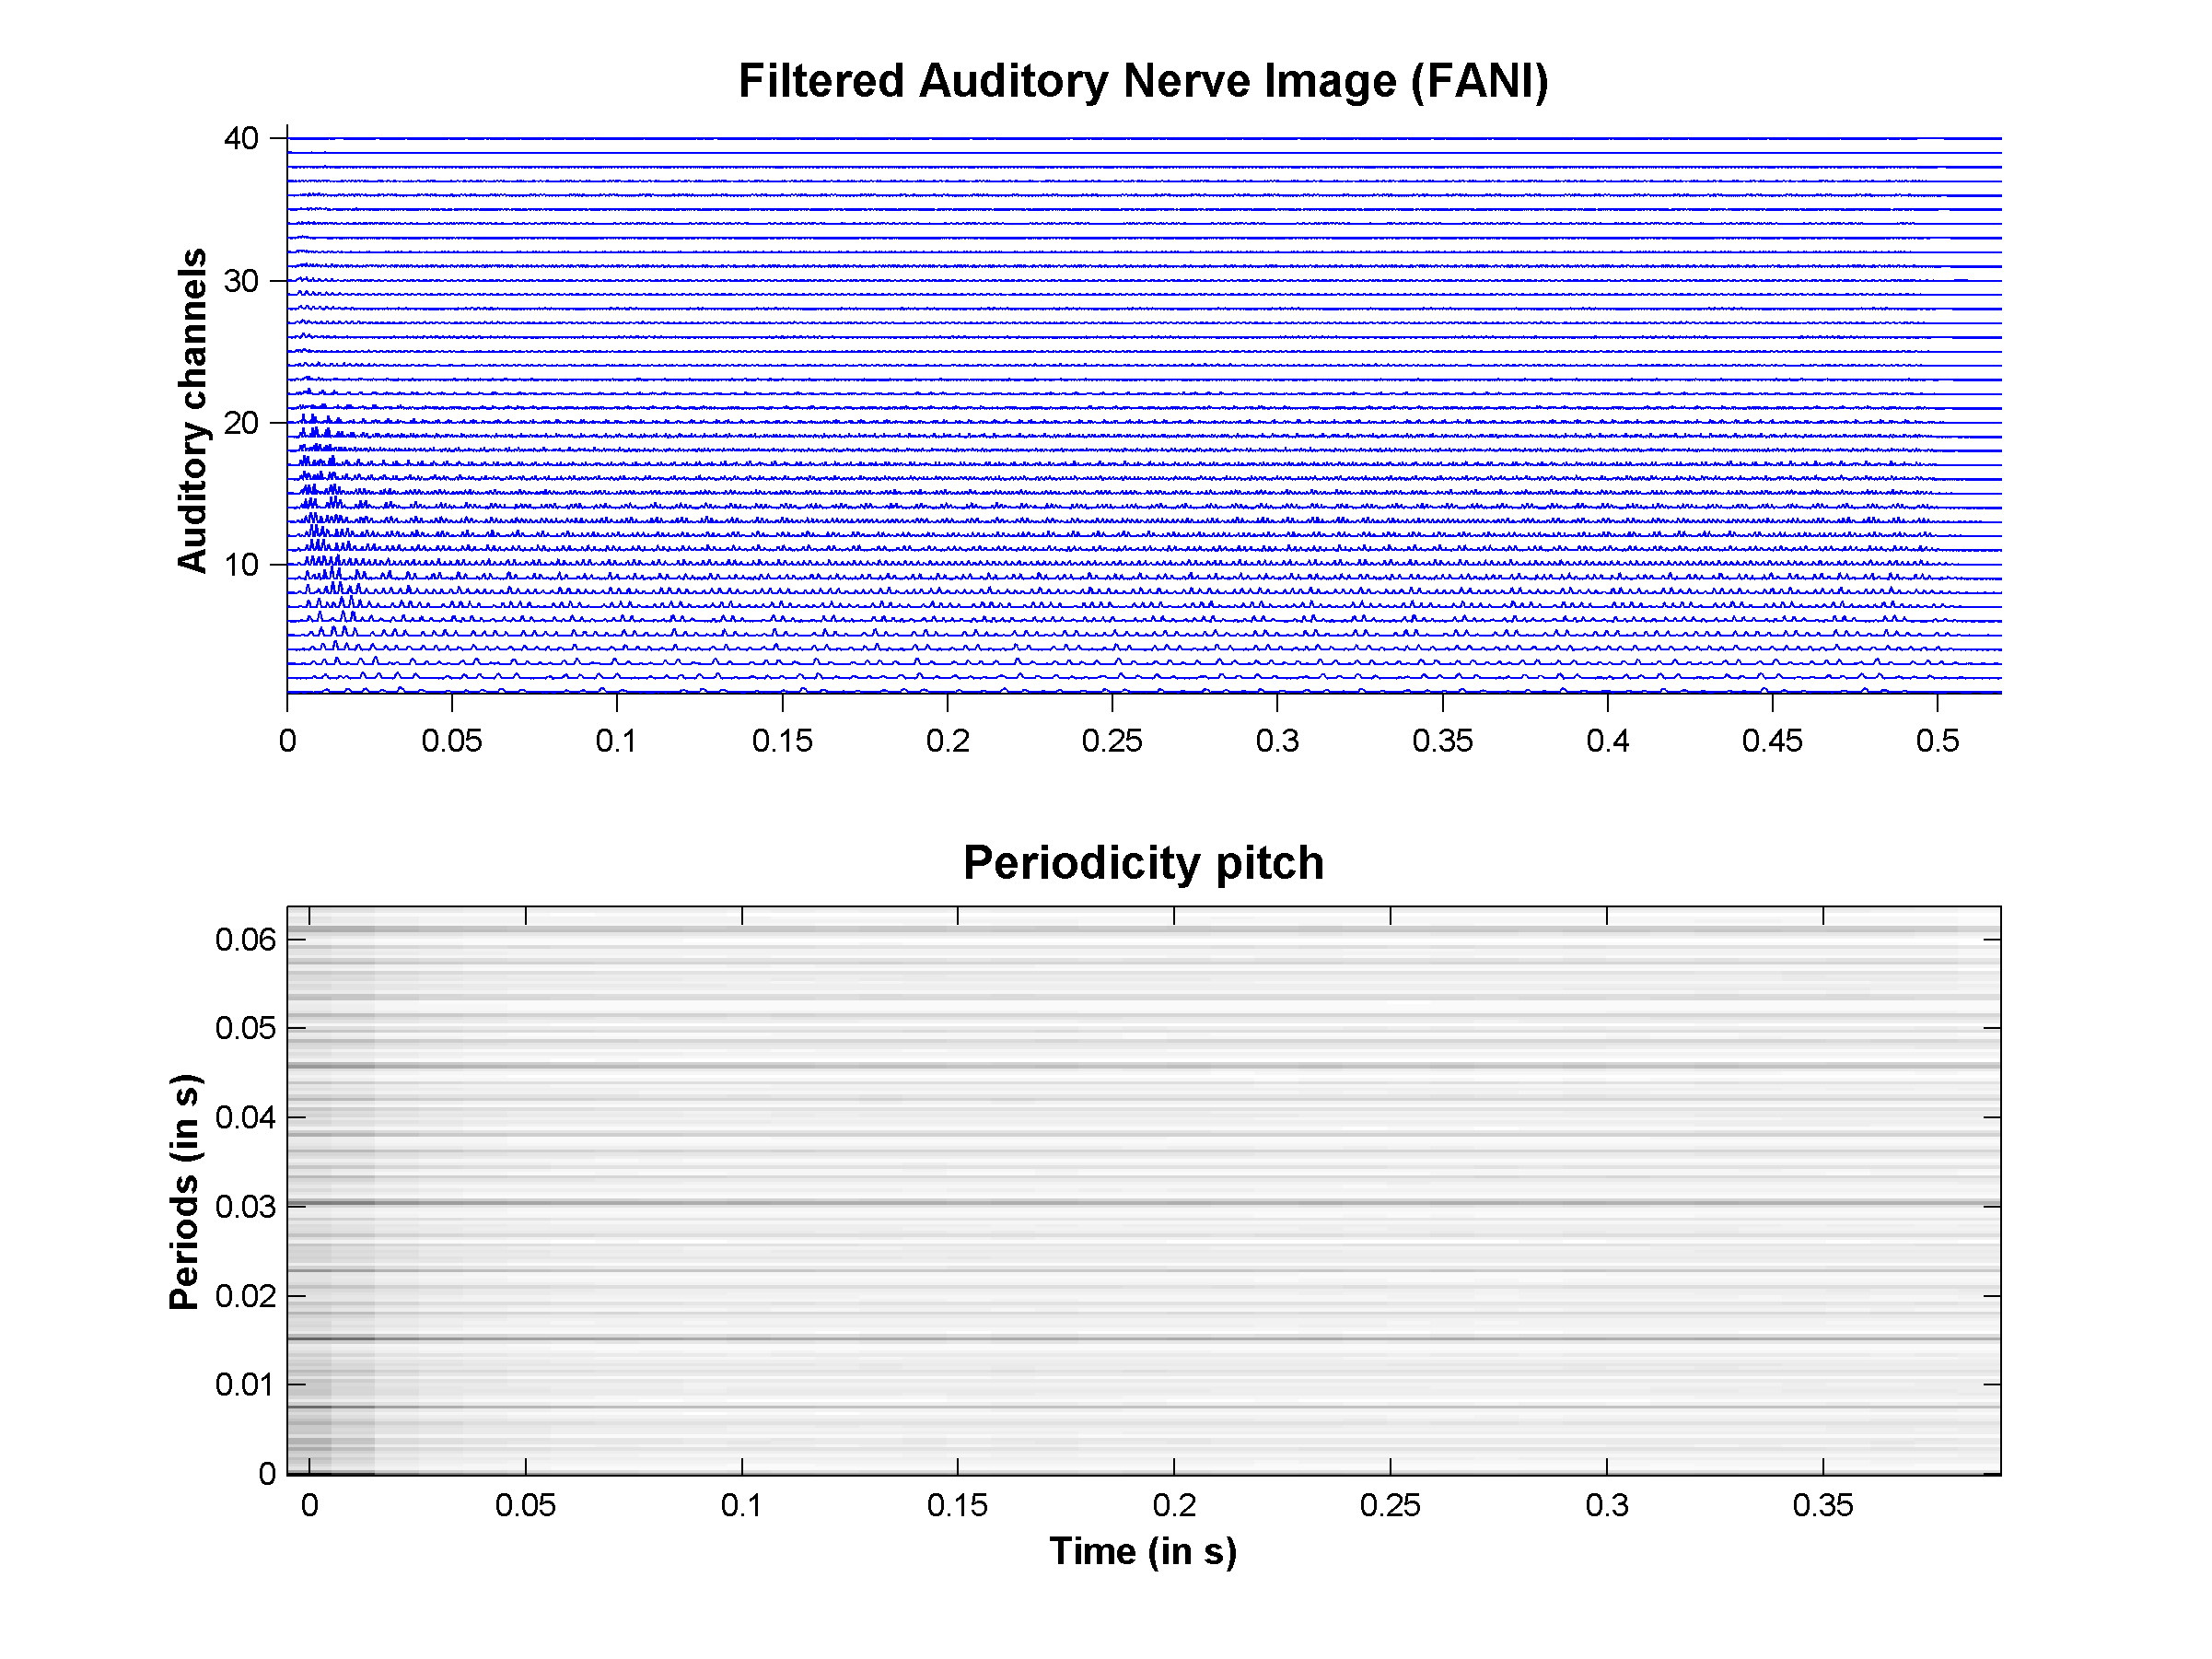
\includegraphics[width=\IPEMDefaultFigureWidth]{Graphics/ShepardCChordPeriodicityPitch}
    \caption{Periodicity Pitch for the C major chord using Shepard tones}
    \label{Fig:ShepardCChordPeriodicityPitch}
\end{figure}
